To address \textbf{RQ1} and \textbf{RQ3} two groups were assigned the task to model a controller for Pacman and Supermario respectively and interview the results afterwards. The first group (Pacman) consists of a subject who is familiar with EmbeddedMontiArc and the second group (Supermario) consists a subjects who have no experience with EmbeddedMontiArc. These groups were selected random among the students of a computer science seminar.
\subsection{Stream Testing (by Heithoff)}

EmbeddedMontiArc comes along with stream tests in order to check a component against a condition as stated in the previous chapter.
We can use those tests to define the conditions the controllers need to fulfill. Those conditions are taken from use cases scenarios. For Pacman the most general acceptance test would be to never let the Pacman die. Due to the fact that stream tests cannot be defined unlimited and that this test might be hard to fulfill the following deterministic tests for Pacman and Supermario were defined.

\subsubsection{Pacman (by Heithoff)}
The tests are taken from use case scenarios as stated before. In this section the process of deriving the stream test from a scenario is presented once and then a few conditions are framed. \newline

\emph{Deriving a Stream Test} \newline
In fig. \ref{fig:PacmanFleeing} a scenario is shown where the only option for Pacman is to flee to the left in order to not collide with the pink and blue ghost. The values of the ghosts and Pacman are partially listed in listing \ref{lst:pmStreamValues}. Together with the other values this concludes to the stream test shown below \ref{lst:pmStreamTest}.
\begin{figure}[!h]
	\centering
	\subfigure[]{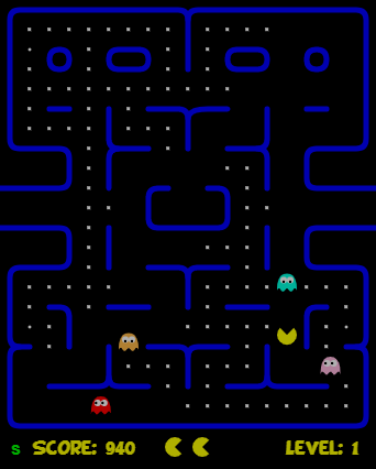
\includegraphics[width=0.49\textwidth]{pictures/Pacman/StreamTests/2/Bild1.PNG}} 
	\subfigure[] {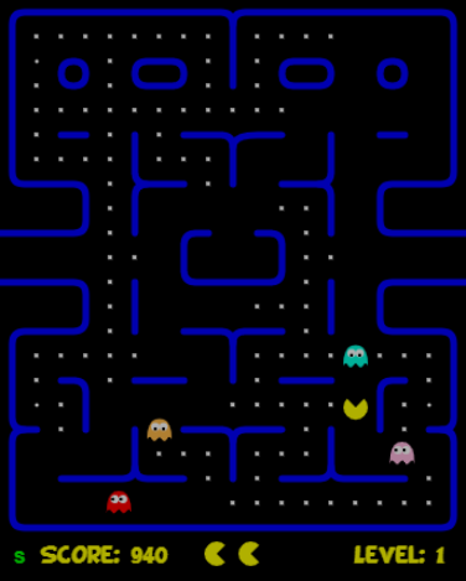
\includegraphics[width=0.49\textwidth]{pictures/Pacman/StreamTests/2/Bild2.PNG}} 
	\subfigure[]{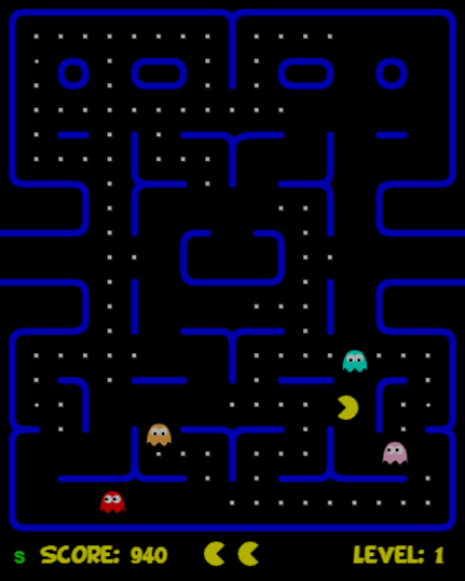
\includegraphics[width=0.49\textwidth]{pictures/Pacman/StreamTests/2/Bild3.PNG}} 
	\subfigure[]{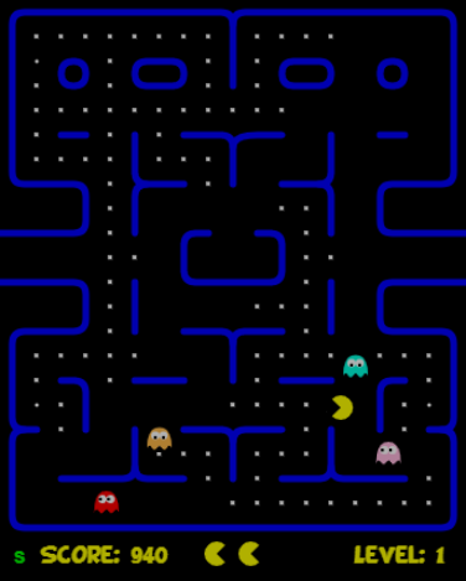
\includegraphics[width=0.49\textwidth]{pictures/Pacman/StreamTests/2/Bild4.PNG}} 
	\caption{Pacman has to move left to avoid colliding with the ghosts} 
	\label{fig:PacmanFleeing}
\end{figure}

\begin{lstlisting}[caption={Values for the stream test},label=lst:pmStreamValues, frame=single, float,floatplacement=H]
(a)
  Pacman: (15m, 17.2m) 
  Pink Ghost: (17m, 19m) 
  BlueGhost: (15m, 14.8m) 
  newDir: 0
(b)	
  Pacman: (15m, 17m) 
  Pink Ghost: (16.8m, 19m) 
  BlueGhost: (15m, 15m) 
  newDir: 0
(c)	
  Pacman: (14.8m, 17m) 
  Pink Ghost: (16.6m, 19m) 
  BlueGhost: (15m, 15.2m) 
  newDir: 2
(d)	
  Pacman: (14.6m, 17m) 
  Pink Ghost: (16.4m, 19m)
  BlueGhost: (15m, 15.4m)
  newDir: 2
\end{lstlisting}

\begin{lstlisting}[caption={Stream test for the scenario above},label=lst:pmStreamTest, frame=single, morekeywords={tick, stream, for, package}, float,floatplacement=H]
package de.rwth.Pacman;
stream Test1 for PacmanWrapper {
  ghostX: [5.4m,15m,17m,7m] tick [5.2m,15m, ...
  ghostY: [21m,14.8m,19m,17.2m] tick [21m,15m, ...
  ghostDirection: [2,1,2,1] tick [2,1,2,1] tick ...
  ghostEtable: [false, false, false, false] tick ...
  ghostEaten: [false, false, false, false] tick ...
  PacmanX: 15m tick 15m tick 14.8m tick 14.6m;
  PacmanY: 17.2m tick 17m tick 17m tick 17m;
  PacmanEaten: false tick false tick false tick false;
  PacmanLives: 3 tick 3 tick 3 tick 3;
  PacmanScore: 0 tick 0 tick 0 tick 0;
  map: [0,0,0,0,0,0,0,0,0,0,0,0,0,0,0,0,0,0,0; ...
  newPacmanDirection: 0 tick 0 tick 2 tick 2;
}
\end{lstlisting}

\emph{Some other tests}\newline
To formulate just some tests, here are a few examples:
\begin{itemize}
	\item If Pacman is located at an intersection and ghosts are coming from two sides, Pacman should walk to a safe path.
	\item If Pacman is located at an intersection and ghosts are at the top path and are all eatable, Pacman should walk this path.
	\item If Pacman is located at an intersection and there are ghosts from 3 directions and in the other direction there is a ghost facing away from Pacman, Pacman should walk this direction.
	\item If there are no ghosts nearby, Pacman should walk the direction with the largest biscuit/coin value.
\end{itemize}

Those scenarios can be tested easily within a few ticks via stream testing.

\subsubsection{Supermario (by Philipp Haller)}
\input{approach-Supermario}

\subsection{Preparations (by Haller and Heithoff)}
The code of the Pacman emulator \cite{PacmanLink} and Supermario emulator \cite{marioLink} is available in HTML5 and JavaScript. C\&C-Components in EmbeddedMontiArc can be translated to C++ code and then to a web assembly \cite{KRSvW18} which uses JavaScript. This JavaScript file can be given inputs according to the component and calculates the outputs on execution. To combine these two files, there is an additional interface needed to extract the information for the inputs out of the emulator and then give the calculated outputs into the emulator.
For the purpose of implementing the controllers the subjects were assigned to use the EmbeddedMontiArcStudio.
EmbeddedMontiArcStudioV1.6.2 did neither support a simulator for Pacman nor a simulator for Supermario. So an additional step to answer RQ2 \textit{Is it possible to integrate other simulators in a recent amount of work} it for the groups to integrate the simulators into the EmbeddedMontiArcStudio.

In order to be able to do so, group Pacman is instructed by an expert (Jean-Marc) which files need modification and what to add. After that this group instructed the second group the same way.

